\documentclass{article}
\usepackage[utf8]{inputenc}
\usepackage[T1]{fontenc}
\usepackage{geometry}
\geometry{margin=1.00in}
\usepackage{hyperref}
\usepackage{xurl}
\usepackage{booktabs}
\usepackage[table]{xcolor}
\usepackage{array}
\usepackage{colortbl}
\usepackage{tikz}
\usetikzlibrary{positioning, shapes.multipart, calc}

\title{API System Documentation: Account and Message Services\\(Spring Boot Refactor)}
\author{Jaehoon Song} 
\date{\today}

\begin{document}

\maketitle

\section{Introduction}
This document provides the formal specifications for the Account and Message management system, acting as the backend for a social media application. It details the HTTP endpoints, expected request formats, business validation logic, database integration patterns, and standardized response structures required for the implementation of the backend services.

\subsection{Architecture}
The system is built utilizing a robust \textbf{3-Layer Architecture}, modernized to leverage the \textbf{Spring Boot Framework}. It utilizes Spring to inject dependencies and autowire functionality using Spring annotations:
\begin{itemize}
    \item \textbf{Controller Layer:} Manages all incoming HTTP requests via Spring Web MVC (e.g., \texttt{@RestController}). It handles routing, automatically parses JSON payloads, and returns formatted JSON responses with corresponding HTTP status codes.
    \item \textbf{Service Layer:} Encapsulates all business logic and strict validation rules. Annotated with \texttt{@Service}, it acts as the intermediary between the controllers and repositories, ensuring data integrity.
    \item \textbf{Repository Layer:} Abstracts all direct database interactions using \textbf{Spring Data JPA} and \texttt{@Repository} interfaces. It replaces raw JDBC and safely executes CRUD operations against the in-memory H2 database.
\end{itemize}

\subsection{Database Entities}
Figure~\ref{fig:uml-erd} shows a compact \textbf{Crow's Foot} (IE) style ERD. The relationships read as follows:
``each \textbf{Message} has exactly one \textbf{Account} (\texttt{postedBy})'' and
``each \textbf{Account} has zero or more \textbf{Message}s''.

\begin{figure}[htbp]
\centering
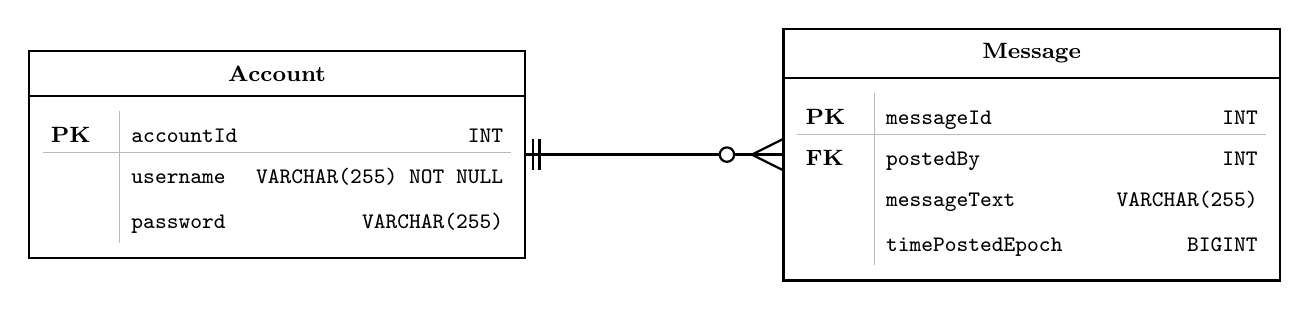
\begin{tikzpicture}[
  font=\footnotesize,
  entity/.style={
    rectangle split,
    rectangle split parts=2,
    draw,
    thick,
    minimum width=6.15cm,
    inner sep=5pt,
    rectangle split part align={center, left},
  },
]
% --- Account ---
\node[entity] (Account) {
  \textbf{Account}
  \nodepart{two}
  {\setlength{\tabcolsep}{2pt}%
   \setlength{\extrarowheight}{2.5pt}%
   \renewcommand{\arraystretch}{1.22}%
   \begin{tabular}{@{\hspace{3pt}}p{8mm}!{\color{gray!55}\vrule width 0.35pt}@{\hspace{4pt}}p{4.72cm}@{\hspace{3pt}}}
  \textbf{PK} & \texttt{accountId}\hfill\texttt{INT}\\
  \arrayrulecolor{gray!55}\hline\arrayrulecolor{black}
   & \texttt{username}\hfill\texttt{VARCHAR(255) NOT NULL}\\
   & \texttt{password}\hfill\texttt{VARCHAR(255)}\\
  \end{tabular}%
  }
};

% --- Message ---
\node[entity, right=3.25cm of Account] (Message) {
  \textbf{Message}
  \nodepart{two}
  {\setlength{\tabcolsep}{2pt}%
   \setlength{\extrarowheight}{2.5pt}%
   \renewcommand{\arraystretch}{1.22}%
   \begin{tabular}{@{\hspace{3pt}}p{8mm}!{\color{gray!55}\vrule width 0.35pt}@{\hspace{4pt}}p{4.72cm}@{\hspace{3pt}}}
  \textbf{PK} & \texttt{messageId}\hfill\texttt{INT}\\
  \arrayrulecolor{gray!55}\hline\arrayrulecolor{black}
  \textbf{FK} & \texttt{postedBy}\hfill\texttt{INT}\\
   & \texttt{messageText}\hfill\texttt{VARCHAR(255)}\\
   & \texttt{timePostedEpoch}\hfill\texttt{BIGINT}\\
  \end{tabular}%
  }
};

% Crow's foot IE: Account end = || (exactly one parent per message); Message end = O + foot (0..* messages per account)
\coordinate (MsgWest) at (Message.west);
\coordinate (Crow) at ($(MsgWest)+(-11pt,0)$);
\coordinate (Ring) at ($(Crow)+(-9pt,0)$);
\coordinate (AccEast) at (Account.east);
% ``||'' sit on the connector just outside Account.east so the spine meets the entity border (no floating gap)
\coordinate (Pipe) at ($(AccEast)+(2.4pt,0)$);
% Horizontal spine: from Account box east anchor through ring to crow vertex
\draw[thick] (AccEast) -- ($(Ring)+(-2.6pt,0)$);
\draw[thick] (Ring) circle[radius=2.6pt];
\draw[thick] ($(Ring)+(2.6pt,0)$) -- (Crow);
% Exactly-one symbol at Account (child references one and only one parent)
\draw[thick] ($(Pipe)+(0,5.5pt)$) -- ($(Pipe)+(0,-5.5pt)$);
\draw[thick] ($(Pipe)+(2.3pt,5.5pt)$) -- ($(Pipe)+(2.3pt,-5.5pt)$);
% Crow's foot opens into Message (many side)
\draw[thick] (Crow) -- ($(MsgWest)+(0,5.5pt)$);
\draw[thick] (Crow) -- (MsgWest);
\draw[thick] (Crow) -- ($(MsgWest)+(0,-5.5pt)$);
\end{tikzpicture}
\caption{Crow's Foot ERD}
\label{fig:uml-erd}
\end{figure}

\noindent\textbf{Physical mapping (H2).} \texttt{accountId} and 
\texttt{messageId} are \texttt{INT} primary keys with 
\texttt{AUTO\_INCREMENT}; \texttt{postedBy} is an \texttt{INT} 
foreign key to \texttt{Account(accountId)}; \texttt{username} is 
\texttt{VARCHAR(255) NOT NULL UNIQUE}.

\subsection{Exception Handling}
The system implements a centralized error handling mechanism using a Controller Advice pattern to ensure consistent HTTP responses. Custom exceptions are mapped to standard HTTP status codes:
\begin{itemize}
    \item \textbf{ClientValidationException:} Mapped to \texttt{400 Bad Request}. Thrown when request payloads fail business validation rules (e.g., blank fields, invalid lengths, or referencing non-existent entities).
    \item \textbf{DuplicateResourceException:} Mapped to \texttt{409 Conflict}. Thrown when attempting to create a resource that violates a unique constraint (e.g., duplicate username).
    \item \textbf{UnauthorizedException:} Mapped to \texttt{401 Unauthorized}. Thrown when authentication credentials are invalid.
\end{itemize}

\newpage
\section{Account Management}

\subsection{User Registration}
A new account is created through a \texttt{POST} request to \path|localhost:8080/register|. 
\begin{itemize}
  \item \textbf{Request Body:} A JSON representation of an Account is provided, excluding the \texttt{accountId}.
  \item \textbf{Success Criteria:} Registration is completed if the username is not blank, the password contains at least four characters, and the username does not already exist in the database.
  \item \textbf{Successful Response:} A status of \texttt{200 OK} is returned. The response body contains the JSON representation of the Account, including the auto-generated \texttt{accountId}. The new account is persisted to the database.
  \item \textbf{Error Handling:} If registration is not successful due to a duplicate username, a \texttt{409 Conflict} status is returned. If the registration fails for any other validation reason, a \texttt{400 Bad Request} (Client Error) status is returned.
\end{itemize}

\subsection{User Login}
Authentication is verified via a \texttt{POST} request to \path|localhost:8080/login|.
\begin{itemize}
  \item \textbf{Request Body:} A JSON representation of an Account is provided, excluding the \texttt{accountId}.
  \item \textbf{Success Criteria:} Login is successful if the provided username and password match an exact, existing record in the database.
  \item \textbf{Successful Response:} A status of \texttt{200 OK} is returned. The response body contains the JSON representation of the authenticated account, including the \texttt{accountId}.
  \item \textbf{Error Handling:} If the login is not successful (credentials do not match any existing account), a \texttt{401 Unauthorized} status is returned.
\end{itemize}

\section{Message Management}

\subsection{Create New Message}
A new post is submitted via a \texttt{POST} request to \path|localhost:8080/messages|.
\begin{itemize}
  \item \textbf{Request Body:} A JSON representation of a message is provided, excluding the \texttt{messageId}.
  \item \textbf{Success Criteria:} The message is persisted if the \texttt{messageText} is not blank, is not over 255 characters, and the \texttt{postedBy} field refers to a real, existing user.
  \item \textbf{Successful Response:} A status of \texttt{200 OK} is returned. The response body contains the complete JSON of the message, including the newly generated \texttt{messageId}.
  \item \textbf{Error Handling:} If the creation of the message is not successful for any reason (e.g., validation failure), a \texttt{400 Bad Request} (Client Error) status is returned.
\end{itemize}

\subsection{Retrieve All Messages}
All messages are retrieved via a \texttt{GET} request to \path|localhost:8080/messages|.
\begin{itemize}
  \item \textbf{Functionality:} Retrieves all posts currently stored in the database.
  \item \textbf{Successful Response:} A status of \texttt{200 OK} is returned. The response body contains a JSON list of all messages retrieved from the database. It is expected for the list to simply be empty (\texttt{[]}) if there are no messages.
\end{itemize}

\subsection{Retrieve Message by ID}
A specific message is retrieved via a \texttt{GET} request to \path|localhost:8080/messages/{messageId}|.
\begin{itemize}
  \item \textbf{Functionality:} Retrieves a single post matching the exact ID path parameter.
  \item \textbf{Successful Response:} A status of \texttt{200 OK} is returned. The response body contains the JSON representation of the identified message. It is expected for the response body to simply be empty if there is no such message.
\end{itemize}

\subsection{Delete Message by ID}
A message is removed via a \texttt{DELETE} request to \path|localhost:8080/messages/{messageId}|.
\begin{itemize}
  \item \textbf{Functionality:} The identified message is permanently removed from the database.
  \item \textbf{Successful Response:} A status of \texttt{200 OK} is returned. If the message existed prior to deletion, the response body should contain the number of rows updated (\texttt{1}). If the message did not exist, the response status should still be \texttt{200 OK}, but the response body should be empty, as the \texttt{DELETE} verb is intended to be idempotent.
\end{itemize}

\subsection{Update Message by ID}
A message text is updated via a \texttt{PATCH} request to \path|localhost:8080/messages/{messageId}|.
\begin{itemize}
  \item \textbf{Request Body:} A JSON payload containing a new \texttt{messageText} value to replace the message identified by the ID. The request body cannot be guaranteed to contain any other information.
  \item \textbf{Success Criteria:} The update is executed if the \texttt{messageId} already exists in the database, the new text is not blank, and the new text length is not over 255 characters.
  \item \textbf{Successful Response:} A status of \texttt{200 OK} is returned. The message stored in the database should have the updated \texttt{messageText}, and the response body should contain the number of rows updated (\texttt{1}).
  \item \textbf{Error Handling:} If the update of the message is not successful for any reason, a \texttt{400 Bad Request} (Client Error) status is returned.
\end{itemize}

\subsection{Retrieve Messages by Account ID}
All messages posted by a specific user are retrieved via a \texttt{GET} request to \path|localhost:8080/accounts/{accountId}/messages|.
\begin{itemize}
  \item \textbf{Functionality:} Filters global messages, returning only those authored by a particular user.
  \item \textbf{Successful Response:} A status of \texttt{200 OK} is returned. The response body contains a JSON list of all messages retrieved from the database posted by the user. It is expected for the list to simply be empty (\texttt{[]}) if there are no messages.
\end{itemize}

\end{document}